\chapter{Approximations}
\label{ch:approximations}
\graphicspath{{../gfx/chapter02/}{../plots/chapter02/}}


\section{Fixed charge model}

Exact diagonalization scales exponentially with system size. With the full
\emph{grand canonical} QCA Hamiltonian \eqref{eq:H_QCA} only devices of up to
two cells are computationally feasible. Therefore, we need to introduce
approximations to access larger systems. Approximating means to simplify.
However, by carefully establishing successive approximations and their limits,
we also reduce the problem to its essential ingredients and thus, hopefully, we
gain a better understanding of the QCA approach. As a first step, we reduce the
Hilbert space to states with a fixed number of particles per cell. We disallow
any charge fluctuations, both for the system as a whole and for each individual
cell. With that, we omit the chemical potential term in the Hamiltonian, $\mu =
0$, and prohibit inter-cell hopping. This is a major simplification. However, it
is in line with the QCA idea: the approach requires a fixed number of charges
per cell, typically two electrons, and cells are thought to interact only via
Coulomb forces. If the \emph{fixed charge} approximation is not valid for a
given system, then there is no hope of implementing QCA on it. For experimental
systems like the atomic silicon quantum dots, it should always be possible, at
least in principle, to tune the system parameters so that for a given cell
layout each cell is occupied by the same number of electrons. The
two-electrons-per-cell sector has to be lowest in energy and other particle
number sectors need to be sufficiently gapped out, that is, at an energy much
larger than temperature. Of course, in practice there are very clear limits as
to how much the system parameters can be tuned. Any QCA cell layout considered
within the fixed charge approximation cannot necessarily be readily implemented
on a given real-world material system.

For the fixed charge model, the state space scales as $N_s = \binom{8}{2}^{N_c}
= 28^{N_c}$ ($N_c$ is the number of cells). Using symmetries, the largest block
of the Hamiltonian matrix is the spin zero sector, of size $N_s^{\prime} =
16^{N_c}$. On conventional computer hardware, systems of up to four cells are
possible, with memory requirements of 32GB. However, such calculations take very
long and therefore three-cell systems are the practical limit.


\section{Bond model}

%
\begin{figure}
  \center
  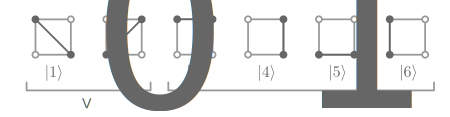
\includegraphics{bond}
  \caption
  [The six bonds of a QCA cell]
  {
  The six bonds of a QCA cell. The basis of a QCA cell in the fixed charge
  picture consists of six bonds and four doubly occupied dots. Each bond
  corresponds to one spin singlet and three spin triplet states. The bond model
  neglects doubly occupied states and keeps only one state per bond for a total
  of six states per cell. From those, the Ising approximation only retains
  the two lowest energy states, $\ket{1}$ and $\ket{2}$ with energy $V_0$.
  }
  \label{fig:bond}
\end{figure}
%
At its heart, QCA is a semi-classical idea. It relies dominantly on
charge-charge interactions and ignores the particle spin. Therefore, as a next
step in our quest to access larger system sizes, we neglect the spin degrees of
freedom. The 28 states of each cell in the fixed charge model can be reorganized
into four doubly occupied dots and six bonds, illustrated in
Fig.~\ref{fig:bond}. Each bond corresponds to one spin singlet and three spin
triplet states. The \emph{bond} approximation only keeps one state for each bond
and discards the doubly occupied states as well. With the bond model we thus
assume that singlet and triplet states are qualitatively and energetically
equivalent, and that doubly occupied dots are sufficiently gapped out, that is,
$U \gg T$. Because QCA ignores the spin, singlets and triplets should be
qualitatively the same---for example, they should yield the same cell
polarizations. However, we can speculate that virtual double-occupancy lowers
the energies of the singlet states and therefore introduces a small
singlet-triplet splitting. Neglecting this small splitting presumably does not
introduce a large error, but we will have to verify this assumption and look at
the splitting in more detail in due course. For the bond model the QCA
Hamiltonian reduces to
%
\begin{equation}
  \label{eq:H_bond}
  H = - \sum_{\left<ij\right>} t c_i^{\dagger} c_j
      + \sum_{i<j} V_{ij} \left( n_i - q \right) \left( n_j - q \right) \, .
\end{equation}
%
With six bond states per cell, the Hilbert space of the bond model is $N_s =
6^{N_c}$ ($N_c$ the number of cells). Five and six cells are doable, with memory
requirements of 460MB and 16GB, respectively, but for practical calculations
five-cell systems really are the limit. For the bond model there are no
symmetries that can be exploited.


\section{Ising model}

%
\begin{figure}
  \center
  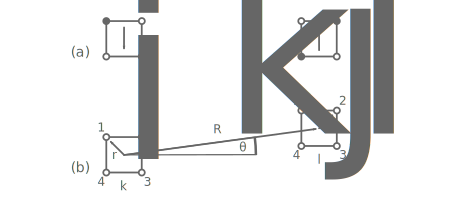
\includegraphics{ising}
  \caption
  [Mapping QCA to an Ising-like model]
  {
  (a) The Ising approximation identifies each cell with a pseudo spin. Logic 0
  corresponds to spin down and logic 1 to spin up. (b) QCA cells $k$ and $l$. 
  }
  \label{fig:ising}
\end{figure}
%
A linear array of QCA cells where each cell has a state of logic 0 or 1 is
reminiscent of a 1D spin $\frac{1}{2}$ chain. Indeed, if we reduce the basis to
only two states per cell, down from six states in the bond picture, we can map
the QCA system to a transverse-field Ising model with long-ranged interactions.
This is an attractive proposition: The smaller Hilbert space allows for larger
system sizes with our exact diagonalization method; more importantly, the
transverse-field Ising model is amenable to sign-problem-free Stochastic series
expansion (SSE) quantum Monte Carlo schemes \cite{Sandvik2003}. These methods do
not scale exponentially\footnote{SSE quantum Monte Carlo methods roughly scale
as $N \ln N$ where $N$ is the system size.} and consequently allow access to
much larger systems. Last, but not least, such a mapping connects the QCA
approach to the established and well studied Ising model. The prospect hinges on
the assumption that the two-states-per-cell basis actually is a good
approximation for QCA systems. And while bistable two-state cells are certainly
the picture we have in mind when we talk about QCA, it is not \emph{a priori}
clear whether this is a correct physical picture. The transverse-field Ising
model is equivalent to the two-states-per-cell approximation that has been used
extensively, but was never satisfyingly derived, in the literature to study the
dynamics of QCA systems.

We use the bond Hamiltonian \eqref{eq:H_bond} as the starting point. We
had already discussed in the last chapter that such a Hamiltonian can be
decomposed into single-cell terms and cell-cell interaction terms,
\begin{equation}
  H = \sum_k H^c_k + \sum_{k<l} H^{cc}_{kl} \, .
\end{equation}
In comparison, the transverse-field Ising model is described by
%
\begin{equation}
  \tilde{H} = - \sum_k \gamma S^x_k + \sum_{k<l} J_{kl} S^z_k S^z_l \, .
\end{equation}
%
Thus, we would like to map the single cell term $H^c_k$ to the transverse-field
term $-\gamma S^x_k$ and the Coulombic cell-cell interaction $H^{cc}_{kl}$ to
the Ising term $J_{kl} S^z_k S^z_l$. Each cell $k$ is identified with a pseudo
spin $S^z_k$, specifically logic 0 with spin down and logic 1 with spin up, as
illustrated in Fig.~\ref{fig:ising}(a). We will first look at how the QCA cell
can be represented by only two basis states and derive an approximate expression
for the transverse field $\gamma$. Then we will use a multipole expansion to
derive $J_{kl}$ from the cell-cell Coulomb interaction.

To arrive at a single-cell-basis with only two states we can, in principle,
follow a similar prescription as for the fixed charge and bond approximations:
we neglect high-energy states which are assumed to be gapped out. In this case,
the neglected states are the four edge states with Coulomb energy $V_1$,
$\ket{\psi_Q} = \left\{ \ket{3}, \ket{4}, \ket{5}, \ket{6} \right\}$,
illustrated in Fig.~\ref{fig:bond}, where we have introduced $\ket{\psi_Q}$ to
denote the high-energy subspace of the single-cell Hilbert space. We only keep
the low-energy diagonal states $\ket{\psi_P} = \left\{ \ket{1}, \ket{2}
\right\}$ with Coulomb energy $V_0$. Of course, these two states are exactly our
logic 0 and logic 1 state, or, in the Ising language, $\ket{\downarrow} \doteq
\ket{1}$ and $\ket{\uparrow} \doteq \ket{2}$. Here, $\ket{\psi_P}$ denotes the
low-energy subspace. For the high-energy states to be sufficiently gapped out,
we require $\Delta V = V_1 - V_0 \gg T$. In contrast to the fixed charge and
bond model, merely truncating the Hilbert space is not sufficient for the Ising
model. For our previous two approximations, the Hamiltonian had remained
essentially unchanged, apart from dropping no longer relevant terms, such as the
chemical potential term or the Hubbard $U$ term. The retained states were
exactly the same states as in the full, untruncated model. But with only two
states per cell the existing Hamiltonian \eqref{eq:H_bond} does not ``work'':
There is no process that takes the cell from $\ket{1}$ to $\ket{2}$ and the
system would be stuck in either of the two spin states eternally. In the bond
picture, in comparison, for the system to transition from state $\ket{1}$ to
$\ket{2}$ it can take different paths, for example $\ket{1} \rightarrow \ket{3}
\rightarrow \ket{2}$, consisting of two hopping processes with an interim
high-energy edge state. We need to derive an effective, low-energy Hamiltonian
from the bond model that treats those processes perturbatively, as
\emph{virtual} excitations, yielding an effective hopping term for the
transition $\ket{1} \leftrightarrow \ket{2}$. This effective hopping is
precisely the transverse field $\gamma$ which flips the spin in the Ising
picture.

A single QCA cell is described by the time-independent Schr\"odinger equation
$H^c_k \ket{\psi} = E_k \ket{\psi}$, with $\ket{\psi} = \left[ \ket{\psi_P}
\ket{\psi_Q} \right]$. Our aim it to truncate the basis to $\ket{\psi_P}$ and
derive an effective Hamiltonian $\tilde{H}^c_k$ with the subspace
Schr\"odinger equation $\tilde{H}^c_k \ket{\psi_p} = E_k \ket{\psi_p}$. Using
the basis depicted in Fig.~\ref{fig:bond}, the single-cell bond Hamiltonian is
very simple and can be written down explicitly. As the single-cell Hamiltonian
is the same for all cells, we can drop the index $k$.
%
\begin{equation}
\begin{split}
  \label{eq:H_marix}
  H^c
  &=
  %
  \left(
  \begin{array}{cc|cccc}
    V_0 & 0   & -t  & -t  & -t  & -t  \\
    0   & V_0 & -t  & -t  & -t  & -t  \\
    \hline
    -t  & -t  & V_1 & 0   & 0   & 0   \\
    -t  & -t  & 0   & V_1 & 0   & 0   \\
    -t  & -t  & 0   & 0   & V_1 & 0   \\
    -t  & -t  & 0   & 0   & 0   & V_1 \\
  \end{array}
  \right) \\[1em]
  %
  &=
  \left(
  \begin{array}{cc}
    H_{PP} & H_{PQ} \\
    H_{QP} & H_{QQ} \\
  \end{array}
  \right)
\end{split}
\end{equation}
%
Here, we have partitioned the Hamiltonian into four blocks, $H_{PP}$, $H_{QQ}$,
$H_{PQ}$, and $H_{QP}$, corresponding to the low-energy subspace $\ket{\psi_P}$,
the high-energy subspace $\ket{\psi_Q}$, and transitioning between the subspaces.
With this partitioned Hamiltonian the time-independent Schr\"odinger equation is
%
\begin{equation}
  \label{eq:SE}
  %
  \begin{pmatrix}
    H_{PP} & H_{PQ} \\
    H_{QP} & H_{QQ} \\
  \end{pmatrix}
  \begin{pmatrix}
    \psi_P \\
    \psi_Q \\
  \end{pmatrix}
  =
  E
  \begin{pmatrix}
    \psi_P \\
    \psi_Q \\
  \end{pmatrix}
  \, .
  %
\end{equation}
%
Writing out the matrix equation as two equations explicitly, and eliminating
$\ket{\psi_Q}$ yields 
%
\begin{equation}
  H_{PP} \ket{\psi_P} + H_{PQ} \frac{1}{E - H_{QQ}} H_{QP} \ket{\psi_P}
  =
  E \ket{\psi_P}
\end{equation}
%
and therefore
%
\begin{equation}
  \label{eq:H_effective}
  \tilde{H}^c = H_{PP} + H_{PQ} \frac{1}{E - H_{QQ}} H_{QP} \, .
\end{equation}
%
Assuming that the system is predominantly in the subspace spanned by
$\ket{\psi_P}$ and additionally that the hopping is very small, $t \ll V_0$, we
can approximate $E \approx V_0$. We write out the matrix multiplications and use
$\left( H_{PP} \right)_{ij} = \left( V_0 \right)_{ii} \delta_{ij}$, $\left(
H_{PQ} \right)_{ij} = \left( -t \right)_{ij}$, and so on. The effective
Hamiltonian becomes
%
\begin{equation}
\begin{split}
  \tilde{H}^c_{ij}
  %
  &=
  \left( V_0 \right)_{ii} \delta_{ij}
  + \left( - t \right)_{ik}
    \left( V_0 - V_1 \right)^{-1}_{kk}
    \left( - t \right)_{kj} \\
  %
  &=
  \left( V_0 \right)_{ii} \delta_{ij}
  - \left( \frac{4 t^2}{\Delta V} \right)_{ij} \, .
\end{split}
\end{equation}
%
As the system remains unchanged upon adding a constant term to the Hamiltonian,
we can subtract the constant diagonal term $\tilde{H}_{ii} = V_0 - \frac{4
t^2}{\Delta V}$, and arrive at
%
\begin{equation}
  \tilde{H}^c
  =
  \begin{pmatrix}
    0 & - \frac{4 t^2}{\Delta V} \\
    - \frac{4 t^2}{\Delta V} & 0 \\
  \end{pmatrix} \, .
\end{equation}
%
The off-diagonal matrix elements are the effective hopping, transitioning the
system between its two states $\ket{1} \leftrightarrow \ket{2}$. If we now
compare this matrix with the transverse-field term of the Ising model,
%
\begin{equation}
\begin{split}
  \tilde{H}^c
  &=
  - \gamma S^x_k \\
  &=
  - \frac{1}{2} \gamma \left( S^+_k + S^-_k \right) \\[0.5em]
  &= 
  \begin{pmatrix}
    0 & - \frac{1}{2} \gamma \\
    - \frac{1}{2} \gamma & 0 \\
  \end{pmatrix} \, ,
\end{split}
\end{equation}
%
we identify the effective hopping as the transverse field $\gamma$,
%
\begin{equation}
  \label{eq:gamma}
  \gamma = \frac{8 t^2}{\Delta V} \, .
\end{equation}
%
The effective hopping is a virtual process involving two hopping processes in
the original bond model, yielding the $t^2$ in the numerator, and an interim
high-energy state gapped out by $\Delta V$, hence the $\Delta V$ in the
denominator. To arrive at the expression for the effective hopping $\gamma$ we
used the assumptions $\Delta V \gg T$ and $t \ll \Delta V$. As a reminder,
$\Delta V = V_1 - V_0 = \frac{2 - \sqrt{2}}{2} \frac{1}{a} \approx 0.3 V_1$.
Notably, the energy gap is independent of the compensation charge $q$. As the
derivation used only a single cell, it is also implicitely assumed that the
perturbations from other cells in the system are small, at least as far as the
effective hopping is concerned. If the hopping depended on the state of nearby
cells, then the effective Hamiltonian would be much more involved and certainly
could not be mapped to an Ising-like model.

We have successfully derived an effective hopping term and therefore also an
effective two-state model for the QCA Hamiltonian. With only two states per cell
the Hilbert space scales as $N_s = 2^{N_c}$ ($N_c$ the number of cells) and up
to 14 cells are computationally feasible, with memory requirements of 2GB. In
practice, we restrict the calculations to a maximum of 12 cells. For our
calculations, we can use the two-state approximation with the effective hopping
term, but still retain the original cell-cell interaction term $H^{cc}_{kl}$.
From a computational point of view, nothing is gained by expressing the
cell-cell interaction as an Ising interaction. However, deriving $J_{kl}$ from
$H^{cc}_{kl}$ is very rewarding conceptually and will already allow some key
insights into the characteristics of QCA devices. Therefore, we now undertake
the derivation of an expression for $J_{kl}$. The obvious starting point is the
cell-cell interaction term $H^{cc}_{kl}$, 
%
\begin{equation}
\begin{split}
  H^{cc}_{kl} 
  %
  &=
  %
  \sum_{\substack{i \in k\\j \in l}} V_{ij} \left( n_i - q \right) \left( n_j - q \right) \\
  %
  H^{cc}_{kl}
  %
  &= 
  %
  \sum_{\substack{i \in k\\j \in l}}
  \frac{ \left( n_i - q \right) \left( n_j - q \right) }
       { \left| \bm{R}_{kl} + \bm{r}_j - \bm{r}_i \right| } \\
  %
  &=
  \sum_{\substack{i \in k\\j \in l}}
  \frac{n_i n_j - q (n_i + n_j)}
       {\left| \bm{R}_{kl} + \bm{r}_{ij} \right|} \, ,
\end{split}
\end{equation}
%
where $i$ and $j$ sum over the four dots $1\ldots4$ of cell $k$ and $l$,
respectively, and $\bm{R}_{kl}$ denotes the vector between the centres of the cells,
see Fig.~\ref{fig:ising}(b). We have introduced $\bm{r}_{ij} = \bm{r}_j -
\bm{r}_i$ and dropped the constant $q^2$ term. There are only four possible
configurations for two interacting cells: $\uparrow\uparrow$,
$\downarrow\downarrow$, $\uparrow\downarrow$, and $\downarrow\uparrow$. Using
the shorthand notations $V_{ij} = \frac{1}{\left| \bm{R}_{kl} + r_{ij} \right|}
+ \frac{1}{\left| \bm{R}_{kl} - r_{ij} \right|}$ and $V_{00} = \frac{1}{\left|
\bm{R}_{kl} \right|}$, we calculate their energies explicitly.
\begin{align}
  %
  E^{\uparrow\uparrow}
  &=
  \left( 1 - 2 q \right) \left( 2 V_{00} + V_{24} \right)
  - q \left( 2 V_{12} + 2 V_{14} \right)
  \\
  %
  E^{\downarrow\downarrow}
  &=
  \left( 1 - 2 q \right) \left( 2 V_{00} + V_{13} \right)
  - q \left( 2 V_{12} + 2 V_{14} \right)
  \\
  %
  E^{\uparrow\downarrow}
  &=
  \left( 1 - 2 q \right) \left( V_{12} + V_{14} \right)
  - q \left( 4 V_{00} + V_{13} + V_{24} \right)
  \\
  %
  E^{\downarrow\uparrow}
  &=
  \left( 1 - 2 q \right) \left( V_{12} + V_{14} \right)
  - q \left( 4 V_{00} + V_{13} + V_{24} \right)
\end{align}
Note that the expression for two spin-down cells can be obtained from the
expression for two spin-up cells (and similarly $E^{\uparrow\downarrow}$ from
$E^{\downarrow\uparrow}$) simply by rotating the system by $90^{\circ}$, or
equivalently, by permuting the dot numbering: $1,2,3,4 \rightarrow 4,1,2,3$.
Symmetries can be exploited, for example $V_{43} = V_{12}$. Evidently,
$E^{\uparrow\downarrow} = E^{\downarrow\uparrow}$, which, given the highly
symmetric geometry of those cell arrangements, does not come as a surprise. But
crucially, we find $E^{\uparrow\uparrow} \ne E^{\downarrow\downarrow}$.
Therefore, we have a system with three distinct energy levels which we cannot
hope to represent with the solely two-level Ising term $J_{kl} S^z_l S^z_l$.
Instead, let us try to map to a \emph{modified} Ising model with a three-level
cell-cell interaction term of the form
%
\begin{equation}
  \label{eq:Ising_term}
  %
  \tilde{H}^{cc}_{kl}
  = 
  J_{kl} S^z_k S^z_l + 
  J^{\prime}_{kl} \left( S^z_k + S^z_l \right) \, .
\end{equation}
%
For this Hamiltonian we have the energies
%
\begin{align}
  \tilde{E}^{\uparrow\uparrow} - \tilde{E}^{\uparrow\downarrow}
  &=
  2J_{kl} + 2J^{\prime}_{kl} \\
  %
  \tilde{E}^{\downarrow\downarrow} - \tilde{E}^{\uparrow\downarrow}
  &=
  2J_{kl} - 2J^{\prime}_{kl}
\end{align}
%
which yields
%
\begin{align}
  \label{eq:Js_from_Es}
  J_{kl}
  &=
  \frac{1}{4} 
  \left( 
    \tilde{E}^{\uparrow\uparrow} + \tilde{E}^{\downarrow\downarrow}
    - 2 \tilde{E}^{\uparrow\downarrow} 
  \right) \\
  %
  J^{\prime}_{kl}
  &=
  \frac{1}{4}
  \left( \tilde{E}^{\uparrow\uparrow} - \tilde{E}^{\downarrow\downarrow} \right) \, ,
\end{align}
%
and therefore, identifying $E^{\uparrow\uparrow} = \tilde{E}^{\uparrow\uparrow},
E^{\downarrow\downarrow} = \tilde{E}^{\downarrow\downarrow}$, and so on,
\begin{align}
  \label{eq:J}
  %
  J_{kl}
  &=
  \frac{1}{4} 
  \left(
    4 V_{00} + V_{13} + V_{24} - 2 V_{12} - 2 V_{14}
  \right) \\
  %
  \label{eq:Jprime}
  %
  J^{\prime}_{kl}
  &=
  \frac{1}{4}
  \left( 1 - 2 q \right)
  \left( V_{24} - V_{13} \right) \, .
\end{align}
These results, while abstract, are remarkable in two ways. First, the newly
introduced term $J^{\prime}_{kl}$ vanished for $q=\frac{1}{2}$. In this case,
$E^{\uparrow\uparrow} = E^{\downarrow\downarrow}$. Thus, for charge neutral
cells we recover the genuine, unmodified transverse-field Ising model. Second,
the Ising $J_{kl}$ itself is independent of the compensation charge $q$. We
will see that $J_{kl}$ is the quadrupole-quadrupole cell-cell interaction, to
leading order. Thus, it is fair to say that $J_{kl}$ is the pure QCA
interaction. With the above equations we can also already look at rotational
symmetries of $J_{kl}$ and $J^{\prime}_{kl}$: $J_{kl}$ is invariant under
rotations by $90^{\circ}$ as can be seen by permuting the dots $1,2,3,4
\rightarrow 4,1,2,3$. This is what we expect intuitively. For example, a
horizontal straight line of cells ($\theta = 0^{\circ}$) should behave exactly
the same as a vertical straight line of cells ($\theta = 90^{\circ}$). In
contrast, $J^{\prime}_{kl}$ is not invariant under rotations by $90^{\circ}$. In
fact, applying the same dot permutation yields $J^{\prime}_{kl}
\xrightarrow{\,\, 90^{\circ}} - J^{\prime}_{kl}$. Consequently,
$J^{\prime}_{kl}$ is symmetric under rotations by $180^{\circ}$. It is also
clear that a non-zero $J^{\prime}_{kl}$ breaks the system's symmetry under spin
rotation---$\tilde{H}^{cc}_{kl}$ is not unchanged for $\uparrow\uparrow \,
\rightarrow \, \downarrow\downarrow$. This has profound implications for QCA.
For non-zero $J^{\prime}_{kl}$ we would, for example, expect different
polarization responses for two spin-down cells versus two spin-up cells, and as
a consequence the device would behave differently for logic 0 and logic 1
signals. From an application point of view, this is definitely not what we want.
For QCA operation we therefore require charge neutral cells and a genuine,
unmodified Ising model.

To obtain more tangible expressions for $J_{kl}$ and $J^{\prime}_{kl}$ we do a
multipole expansion of the $V_{ij}$ terms. Specifically,
%
\begin{equation}
\begin{split}
  \frac{1}{\left| \bm{R}_{kl} \pm r_{ij} \right|}
  &=
  \frac{1}{R_{kl}}
  \left( 
  1 \pm 2 \frac{\bm{r}_{ij} \hat{\bm{R}}_{kl}}{R_{kl}} + \frac{r_{ij}^2}{R_{kl}^2}
  \right)^{-1/2} \\
  &=
  \frac{1}{R_{kl}} \left( 1 \pm x + y \right)^{-1/2}
\end{split}
\end{equation}
%
is Taylor-expanded in $x$ and $y$, keeping all terms up to
$\mathcal{O}\left(\frac{a^4}{R_{kl}^5}\right)$, which corresponds to
quadrupole-quadrupole interactions. Plugging the results of the expansion back
into Eqs.~\eqref{eq:J} and \eqref{eq:Jprime} yields
%
\begin{align}
  \label{eq:J_}
  %
  J_{kl}
  &=
  \frac{ 1 }{ 32 }
  \left(
    9 - 105 \cos{4 \theta}
  \right)
  \frac{ a^4 }{ R_{kl}^5 }
  \\
  %
  \label{eq:Jprime_}
  %
  J^{\prime}_{kl}
  &=
  \left( 1 - 2 q \right)
  \left(
    \frac{ 3 }{ 2 } \sin{2 \theta} \frac{ a^2 }{ R_{kl}^3 } +
    \frac{ 5 }{ 4 } \sin{2 \theta} \frac{ a^4 }{ R_{kl}^5 }
  \right) \, .
  %
\end{align}
%
The leading order term of $J_{kl}$ is $R^{-5}$, the quadrupole-quadrupole
interaction. In contrast, the leading order term of $J^{\prime}_{kl}$ is
$R^{-3}$ and therefore, in general, $J^{\prime}_{kl}$ would be the dominating
term---yet another argument why a non-zero $J^{\prime}_{kl}$ is highly
undesirable for functioning QCA devices. Of course, we find our general symmetry
observations confirmed by these more concrete expressions for $J_{kl}$ and
$J^{\prime}_{kl}$: the former is invariant under $90^{\circ}$ rotations, the
latter only under rotations of $180^{\circ}$. Both terms vanish at select
angles. For example, we have $J^{\prime}_{kl} = 0$ for $\theta = 0^{\circ}$, so
that at least for an exactly straight line of cells we recover the unmodified
Ising model, even for non-charge-neutral cells. This does not help when building
more complex devices than a wire, of course, but might still be useful for some
experiments. As another example, $J_{kl} = 0$ for $\theta = 22.5^{\circ}$.
Conceivably, this could be exploited for device applications, to decouple
closely spaced cells. As multipole expansions, the obtained expressions for
$J_{kl}$ and $J^{\prime}_{kl}$ should be valid for large cell-cell distances. In
principle, an arbitrary number of higher order terms can be included to make the
expressions as exact as desired. In practice on the computer, however, we do not
use the multipole expansion at all, but simply sum up all Coulomb interactions
exactly. We will see in due course that for the small cell-cell distances that
we are typically interested in, an expansion up to $R^{-5}$ is indeed not
sufficient, and higher order terms would have to be included.

In summary, we have successfully mapped the QCA bond
Hamiltonian \eqref{eq:H_bond} to a modified transverse-field Ising model,
\begin{equation}
  \label{eq:H_Ising}
  %
  \tilde{H}
  =
  - \sum_k \gamma S^x_k
  + \sum_{k<l}
    \left[
      J_{kl} S^z_k S^z_l + 
      J^{\prime}_{kl} \left( S^z_k + S^z_l \right)
    \right] \, ,
\end{equation}
where $J_{kl}$ and $J^{\prime}_{kl}$ are given by Eqs.~\eqref{eq:J_} and
\eqref{eq:Jprime_}, and $\gamma$ by Eq.~\eqref{eq:gamma}.


\section{Validity of the approximations}
\label{sec:validity_of_the_approximations}

In the last three sections we have introduced three successive approximations
for the QCA Hamiltonian: the fixed charge model, the bond model, and the Ising
model. However, even though we know the theoretical limits in which those
approximations become exact, we have given little thought to the practical
limits. Numerical benchmarks will help us establish the parameter regimes where
we can use the approximations and get sufficiently accurate results, and also
give us a better understanding of how the approximations behave in those
parameter ranges.

%
\begin{figure}
  \center
  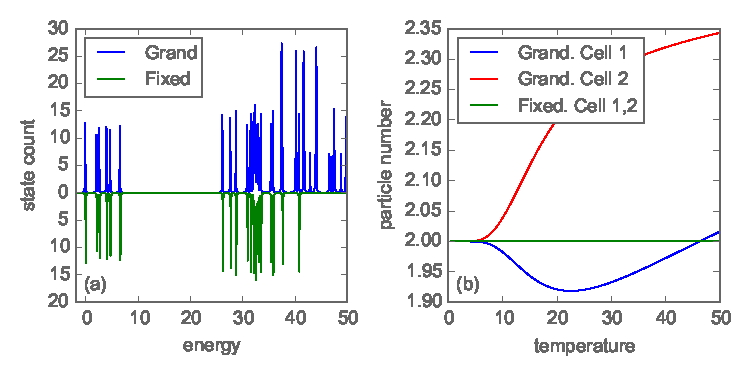
\includegraphics{fixed_charge_approximation}
  \caption
  [The fixed-charge approximation]
  {
  (a) Low-energy density of states of the exact grand canonical and the
  approximative fixed charge two-cell QCA system. For small energies the curves
  agree perfectly (up to $E \lesssim 35$). (b) Particle number per cell over
  temperature for the same two-cell system. The curves diverge for $T \gtrsim
  10$.
  }
  \label{fig:fixed_charge_approximation}
  % parameters: V_1 = 100, boa = 2, U = 1000, mu = 250, 2 cells, q = 0
\end{figure}
%
%
\begin{figure}
  \center
  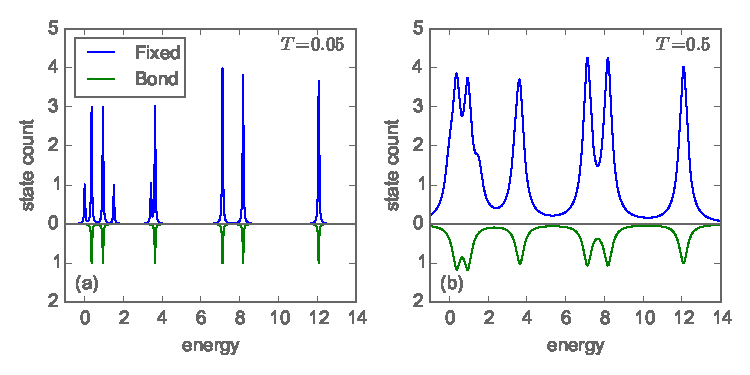
\includegraphics{bond_approximation1}
  \caption
  [The bond approximation for a one-cell system]
  {
  (a) Low-energy density of states of a one-cell QCA system for both the fixed
  charge and the bond model. The bond approximation only reproduces the triplet
  states, but omits the singlet states. The ``measurement'' temperature is
  indicated. (b) The same spectrum, but ``measured'' at a higher temperature.
  The singlet-triplet splitting is ``washed out'' at large enough temperatures:
  the singlet and triplet peaks are no longer separately resolved and each bond
  model state corresponds to four fixed charge states at roughly the same
  energy.
  }
  \label{fig:bond_approximation1}
  % parameters: V_1 = 20, boa = 2, U = 1E6, q = 0, P_D = 1, T = 1, mu = 0
\end{figure}
%
The fixed charge approximation is a Hilbert space truncation where we only keep
the states with exactly two electrons per cell.
Fig.~\ref{fig:fixed_charge_approximation}(a) compares the density of states of
the fixed charge model against the exact grand canonical model for a two-cell
system. The chemical potential is $\mu = 250$ and the nearest-neighbour Coulomb
energy is $V_1 = 100$, whereas the on-site Coulomb repulsion is $U = 1000$. The
energies are in units of the hopping $t$, with $t = 1$. The cells are placed a
distance $d/a = 3$ apart, horizontally. This system does not have any
compensation charges, hence $q = 0$. The approximation reproduces the low-energy
spectrum exactly, in the plot up to $E \lesssim 35$. Therefore, as long as the
two-electrons-per-cell sector is lowest in energy and the temperature is small
compared to the energy of the next charge sector, the model works perfectly.
Fig.~\ref{fig:fixed_charge_approximation}(b) plots the number of particles per
cell over temperature and demonstrates the breakdown of the approximation.
Whereas the fixed charge model gives, per definition, a constant number of
particles over the whole temperature range, the grand canonical system's cell
occupancies start to diverge from two electron per cell at around $T \sim 10$.
This roughly corresponds to the energy states the fixed charge model misses at
$E \gtrsim 35$. A small deviation from exactly two electrons per cell is not
detrimental to QCA, a cell occupied by only one or by three electrons, however,
renders QCA non-functional. We often use the fixed charge model as the starting
point and assume, without further investigation, that a practical QCA
implementation can be tuned to be in the right charge regime at a given
temperature.

The bond model neglects doubly occupied states and represents the four states of
a bond---one singlet and three triplets---with only one single bond state. The
model thus assumes that singlet and triplet states are energetically equivalent,
but we had already asserted that we might expect a small singlet-triplet
splitting. Fig.~\ref{fig:bond_approximation1}(a) shows the density of states of
a single QCA cell for both the fixed charge and the bond model. The hopping is
again $t=1$, the nearest-neighbour Coulomb energy is $V_1 = 20$, and the on-site
Coulomb repulsion is $U = 10^6$---practically at infinity. A driver cell placed
at a distance $d/a = 3$ to the left of the single cell sets an input. We have
chosen the driver cell's polarization to be $P_D = 1$. Indeed, each bond state
corresponds to three fixed charge states---the triplet---and one ``close-by''
state---the singlet. They are not energetically equivalent, but split by a small
energy gap, $\Delta E_S$, the singlet-triplet splitting. Like the fixed charge
model, the bond approximation truncates the Hilbert space and the retained
states are exact. Evidently, the bond model keeps one triplet state, but
discards the other two and the singlet. We speculate that, similar to the
antiferromagnetic Heisenberg coupling constant $J$ emerging in the low-energy
limit of the Hubbard model (with $J \sim \frac{t^2}{U}$) \cite{Auerbach}, here,
virtual excitations to high-energy doubly occupied states lower the energy of
the singlet state and make it the ground state. Because the bond model misses
those doubly occupied states, it cannot accommodate singlet states and hence
reproduces the triplet states. Consequently, we cannot hope that the bond model
is correct for ground state and low-temperature properties. We assert that as
long as the singlet-triplet splitting is ``washed out'', that is, as long as the
temperature is much larger than the singlet-triplet gap, $T \gg \Delta E_S$, the
approximation should give good results. At high enough temperatures, the system
no longer ``sees'' the difference between the singlet and the triplet states.
This is illustrated in Fig.~\ref{fig:bond_approximation1}(b) where the spectrum
is ``measured'' at a higher temperature:%
%
\footnote{
We calculate the density of states graphs by folding the energy
eigenvalues of the system---a delta function energy spectrum---with a Lorentzian
with the half-width at half-maximum set by a ``measurement'' temperature. Very
roughly speaking, this corresponds to a photoemission / inverse photoemission
spectroscopy experiment at this temperature.
}%
%
the singlet and triplets are no longer resolved separately. Instead, each bond
state corresponds to four fixed charge states at roughly the same energy.

The figure shows all six bond states of the single cell---the complete spectrum
apart from the doubly occupied states. As this cell is perturbed by a nearby
driver cell with $P_D = 1$, the ground state is qualitatively closest to the
logic 1 state, or $\ket{2}$ in Fig.~\ref{fig:bond}. Similarly, the first excited
state is similar to $\ket{1}$, or logic 0, and the four higher energy states
correspond to $\ket{4}$, $\ket{5}$, $\ket{3}$, and $\ket{6}$, in that order. Of
course, in general the energy eigenstates are a mixture of all basis states, but
we can still characterize them by the most dominantly contributing basis state.
As this is a non-charge-neutral system, $q=0$, with a relatively small cell-cell
distance $d/a = 3$, charge buildup tends to push the electrons to the far edge
of the cell, thus making $\ket{4}$ lower in energy than $\ket{6}$.

Since the bond model ignores the singlet-triplet splitting, it is important to
understand how the gap $\Delta E_S$ depends on various system parameters. To
that end we picked out a few selected singlet-triplet states from the spectrum
in Fig.~\ref{fig:bond_approximation1}(a) as examples. Contrary to expectations,
for those states the gap $\Delta E_S$ did not change significantly with the
on-site Coulomb repulsion $U$. However, it did become smaller for shorter and
shorter cell-cell distances $d$. Most importantly, for the nearest-neighbour
Coulomb energy $V_1$ we found $\Delta E_S \sim \frac{1}{V_1^p}$. The exponent is
$p \sim 3$ when the cell ``sees'' a biasing external potential (e.g.\ $P_D = \pm
1$) and $p \sim 1$ otherwise (e.g.\ $P_D = 0$). Even though our method is
anything but rigorous and the obtained results very likely not universally true,
the findings should nonetheless give a good enough idea of the principal trends.
Quite generally, the higher the overall Coulomb potential---large $V_1$ and small
$d$---the smaller the singlet-triplet splitting and, conceivably, the more
accurate the bond approximation. The bond model should work as long as $T
\gg T_{min}$ with $T_{min} \sim \Delta E_S$, and as a very rough guideline we can
use $\Delta E_S \sim \frac{t^2}{V_1}$. Of course, we also need $T \ll T_{max}$
with $T_{max} \sim U$, so that the doubly occupied states are gapped out.

%
\begin{figure}
  \center
  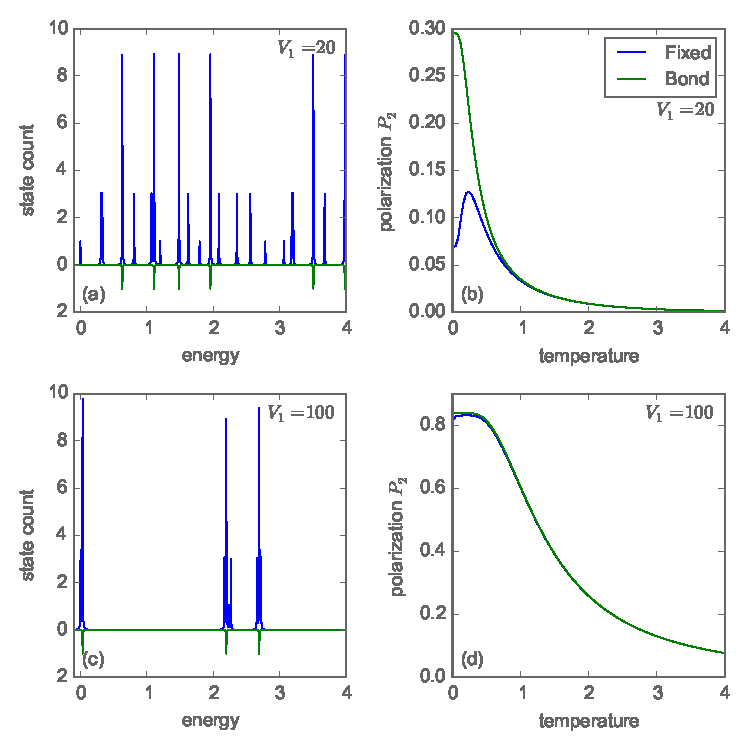
\includegraphics{bond_approximation2}
  \caption
  [The bond approximation for a two-cell system]
  {
  The two-cell fixed charge and bond systems at $V_1 = 20$ and $V_1 = 100$.
  (a)(c) Low-energy density of states. (b)(d) Output polarization $P_2$ over
  temperature. For a small Coulomb repulsion the density of states curves look
  qualitatively very different (a) and the bond approximation does not work very
  well (b). At a larger Coulomb repulsion the density of states curves look much
  more alike (c) and the bond approximation works much better (d).
  }
  \label{fig:bond_approximation2}
\end{figure}
%
To illustrate the limitations of the bond approximation we now look at a
two-cell system: a horizontal line of cells with two active cells and a driver
cell to the left. Fig.~\ref{fig:bond_approximation2} shows the spectra and
output polarizations of the system for two different Coulomb energies, $V_1 =
20$ and $V_1 = 100$. Otherwise the parameters are the same as for the one-cell
system in the previous graph. In particular, the spectrum in
Fig.~\ref{fig:bond_approximation2}(a) is exactly the same as in
Fig.\ref{fig:bond_approximation1}(a), except that we have added one more cell to
the system. Each bond state now corresponds to 16 ($4 \cdot 4$) fixed charge
states. Looking at the four lowest-energy peaks in the spectrum, we see that the
bond model exactly reproduces the nine triplet-triplet states, but misses the
three singlet-triplet and the three triplet-singlet states (in the graph the
corresponding two peaks are hardly distinguishable), as well as the single
singlet-singlet ground state. The four lowest bond states should roughly
correspond to, in that order, both cells being aligned with the driver cell (the
ground state), only one of the two cells being aligned with the driver cell, and
both cells being anti-aligned with the driver cell. Higher energy states have at
least one of the cells not in the preferred diagonal states, $\ket{1}$ and
$\ket{2}$, with electrons occupying predominantly the edge of a cell.

Arguably, the spectra of the fixed charge and the bond model in
Fig.~\ref{fig:bond_approximation2}(a) do not look very similar. Consequently,
the polarization curves in Fig.~\ref{fig:bond_approximation2}(b) do not agree,
especially at low temperatures. In fact, it is rather remarkable that given the
widely dissimilar spectra, the polarizations actually do agree relatively well
at higher temperatures, $T \gtrsim 1$. The bond model only reproduces the most
populous energy states of the exact spectrum. Apparently, that is enough to give
(almost) correct results at high temperatures. The lower the temperature, the
more important become the few lowest lying energy states which the bond model
misses. Very roughly speaking, the temperature where the bond model's
polarization becomes accurate also matches the temperature where we saw the
singlet-triplet splitting being washed out in
Fig.~\ref{fig:bond_approximation1}(b). For the much larger Coulomb energy $V_1 =
100$ the spectra look much more alike, qualitatively, even though the bond model
obviously still does not resolve all the lines of the exact density of states,
as illustrated in Fig.~\ref{fig:bond_approximation2}(c). Therefore, the
approximation works much better: the polarization curves agree down to much
lower temperatures and even the discrepancy of the ground state polarizations is
much reduced, as demonstrated in Fig.~\ref{fig:bond_approximation2}(d).
Compared to the $V_1 = 20$ system, the ground state polarization is much larger
and, generally, the larger the cell polarization, the better the agreement
between bond and fixed charge model. We also note that in the spectrum the peaks
are much more spaced out and thus the $V_1 = 100$ wire retains larger cell
polarizations up to much higher temperatures. For any conventional material, a
Coulomb energy scale such as we have chosen here, $V_1/t \ge 20$, where we have,
of course, $U/t \gg V_1/t$, seems like an extremely large value. However, we
will find that such Coulomb energies are generally in agreement with what the
QCA approach itself requires, and we will discuss this in detail in the next
chapter.

The polarization of the fixed charge model shows a curious bump at low
temperatures, for example in Fig.~\ref{fig:bond_approximation2}(b), and
similarly, if less visibly, in Fig.~\ref{fig:bond_approximation2}(d).
Apparently, the ground state is not the most polarized state. Maximum
polarization is reached at a small, but finite temperature. At the same time,
for the bond model the ground state is the most polarized state and generally
its zero-temperature polarization is larger than that of the fixed charge model.
Interestingly, in contrast to the fixed charge model the bond model's ground
state polarization is largely independent of the magnitude of the driver
polarization and also only weakly influenced by the cell-cell distance $d$,
especially for charge-neutral cells where no charge buildup occurs. Instead, it
is predominantly set by $V_1$, and thus by $V_1/t$ and the energy gap $\Delta V
= V_1 - V_0$. Without an external perturbation such as a non-zero driver
polarization the ground state polarization is zero, of course. But any
infinitesimal external perturbation will instantly see the bond model's ground
state become almost fully polarized. We interpret this behaviour as the ground
state actually consisting of two energetically degenerate states, corresponding
to $\pm P_{gs}$, where $P_{gs}$ is the full ground state polarization for a
given $V_1$. The smallest perturbation lifts this degeneracy and sees the system
snapping to either $+P_{gs}$ or $-P_{gs}$. Now the bond model's ground state
corresponds to the fixed charge model's triplet state---one of the lower lying
excited states, but not the ground state. The true ground state of the more
exact model is a single singlet state, a superposition of the $+P_{gs}$ and
$-P_{gs}$ (and other) states. Therefore, the polarization of the true ground
state is generally smaller in magnitude than the polarization of the
corresponding two triplet states, explaining the low temperature bump in the
polarization curve and the larger polarization of the bond model's ground state.

%
\begin{figure}
  \center
  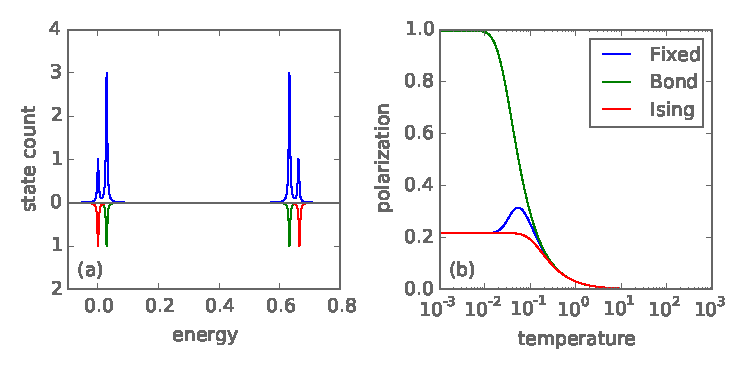
\includegraphics{ising_approximation1}
  \caption
  [The Ising approximation for a one-cell system]
  {
  Comparing the fixed charge, bond, and Ising model for the one-cell
  charge-neutral QCA system. (a) Low-energy density of states. The Ising model
  reproduces the singlet and not the triplet states, as the bond model does. (b)
  Cell polarization over temperature. At larger temperatures $T \gtrsim 0.3$ all
  three models seem to agree. At $T = 0$ the bond model is wrongly fully
  polarized, whereas the Ising model exactly reproduces the fixed charge model's
  ground state polarization.
  }
  \label{fig:ising_approximation1}
  % parameters: V1 = 100, boa = 3, P_D = 0.1, q = 0.5
\end{figure}
%
The Ising approximation is derived as an effective low-energy model from the
bond Hamiltonian. It is therefore qualitatively different from the previous two
approximations: it is not merely a Hilbert space truncation. While the Ising
model should resemble the bond model in the limit where the approximations in
its derivation become exact, for less than optimal parameters the models' states
need not be in perfect agreement. The derivation assumed $E \approx V_0$ ($E$
the energy of the whole system) and therefore $t \ll \Delta V$ as well as $T \ll
\Delta V$. Additionally, cells were assumed to be isolated, so the Ising model
presumably requires reasonably large cell-cell distances. Naturally, the model
inherits the limits of the bond approximation, and we would therefore expect $T
\gg \Delta E_S$ ($\Delta E_S$ the singlet-triplet splitting) and $T \ll U$ as
further requirements. It is important to keep in mind that the Ising model is
not a low-energy model for the more exact fixed charge Hamiltonian---it is
derived as the low-energy limit of the bond model, which, however, is not an
accurate low-energy description of the fixed charge system. The approximation
can also not hope to capture non-charge-neutral systems correctly. It simply
lacks the edge states that are the manifestation of charge buildup, as discussed
in the example of the one-cell bond system above. We had seen in the derivation
of the Ising model that non-charge-neutral cells are very problematic for the
QCA approach in general. Consequently, we will concentrate on charge-neutral
systems with a compensation charge $q = \frac{1}{2}$ for the remainder of the
chapter.

To understand how the Ising approximation behaves, we again start by looking at
the density of states of a one-cell system, shown in
Fig.~\ref{fig:ising_approximation1}(a). We have plotted both the fixed charge
and bond model's density of states for comparison and now use slightly different
system parameters: the nearest-neighbour Coulomb energy is $V_1 = 100$, the
cell-cell distance is $d/a = 4$, and the driver cell is only slightly polarized
with $P_D = 0.1$. As always, the hopping is $t=1$. We are in for a surprise!
Evidently, the Ising model reproduces the singlet states and not the bond
model's triplet states. In line with this observation, the Ising model exactly
matches the fixed charge model's ground state polarization, but misses the
triplet-bump at $T \sim 0.05$, as can be seen in
Fig.~\ref{fig:ising_approximation1}(b). Here, for the charge-neutral system,
the bond model's ground state is fully polarized even at this large cell-cell
distance and for a very weak driver cell polarization. Even though we had
derived the Ising model from the bond Hamiltonian, it does not resemble the bond
model at all, which is very confusing. To lift the confusion, we first note
that, even though the Ising model correctly captures the fixed charge ground
state of the single-cell system, this is not true in general for larger systems,
as we will see in a moment. Second, we need to be very careful when we talk
about the bond model. The bond Hamiltonian is simply a spinless model that does
not distinguish between singlet and triplet states. In contrast, the bond model
uses a concrete basis and we saw that it chooses the triplet states. Therefore,
the bond Hamiltonian, from which we derived the Ising model, and the bond model
are not equivalent. Because the Ising model is an effective low-energy model, it
makes sense that it captures the singlet states, which are lowest in energy. The
Ising and bond states should still eventually become energetically and
qualitatively equivalent, in the limit where the Ising model becomes exact and
the singlet-triplet splitting goes to zero. On second thought, the fact that the
Ising model exactly reproduces the ground state of the one-cell system is maybe
not as surprising, because we had derived it precisely for a single, isolated
cell.

Close inspection of the Ising model's only two states as compared to the
equivalent fixed charge model's states show that they are not exactly the same
energetically. The difference is hardly discernible in the plotted spectrum, but
more pronounced for differently chosen system parameters. Given that the Ising
approximation is an effective model and used several assumptions in its
derivation, this is hardly surprising. For the single-cell system we can easily
study the error of the energies of the Ising states with respect to the fixed
charge states: the states are in better agreement for larger $V_1$ and smaller
$t$. The error explodes for very small cell-cell distances $d/a < 2$---when the
assumption of isolated cells breaks down---but is largely independent of $d/a$
otherwise. Therefore, we find the assumptions and limits of the derivation
confirmed.

To be able to better quantitatively compare different models we introduce the
relative error of the polarization, defined as
%
\begin{equation}
  \epsilon^I_k = \frac{\left|P^F_k - P^I_k\right|}{P^F_k}
\end{equation}
%
for the Ising model. We use the fixed charge model as the reference. Hence,
$P^F_k$ refers to the polarization of cell $k$ with the fixed charge
model and $P^I_k$ is the same polarization, but determined using the Ising
model. The relative error for the bond model, $\epsilon^B_k$, is defined
equivalently. The relative error is independent of the magnitude of the
polarization and therefore suitable for comparing models over wide parameter
ranges. For best results it is also desirable to not drive the systems
into full polarization. Once cells are saturated at $\left| P_k \right| \sim 1$
the quantitative differences between the models disappear. This is why for our
calculations with the Ising model here, which generally require larger $V_1/t$
ratios, we have chosen larger cell-cell distances and smaller driver cell
polarizations, resulting in less polarized cells.

%
\begin{figure}
  \center
  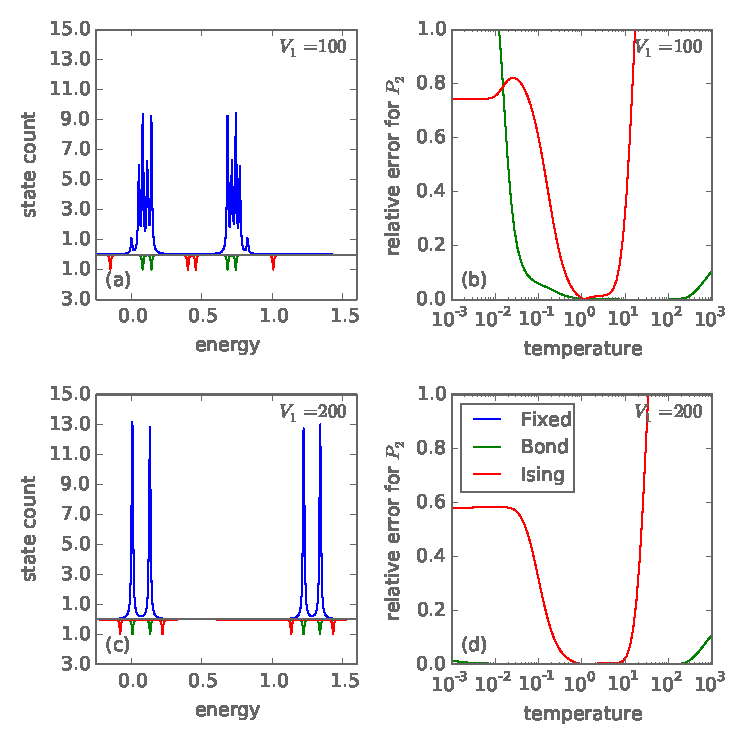
\includegraphics{ising_approximation2}
  \caption
  [The Ising approximation for a two-cell system]
  {
  Comparing the fixed charge, bond, and Ising model for the two-cell
  charge-neutral QCA system at $V_1 = 100$ and $V_1 = 200$. (a)(c) Low-energy
  density of states. The Ising model's spectrum is qualitatively quite wrong,
  although it is in better agreement with the bond model's spectrum for larger
  $V_1$. (b)(d) Relative error of the output polarization of the bond and Ising
  model, with respect to the fixed charge model. The bond model's error is small
  over a large range of temperatures. At $T \sim U \sim 1000$ the neglected
  doubly occupied states become noticeable. The Ising model's error is small
  only over a relatively narrow temperature range. Its ground state no longer
  agrees with the fixed charge model's ground state.
  }
  \label{fig:ising_approximation2}
  % parameters: V1 = 100, 200, boa = 3, P_D = 0.1, q = 0.5, U=1E3
\end{figure}
%
Fig.~\ref{fig:ising_approximation2} shows the relative error over temperature
together with the density of states for all three models for a two-cell system
at $V_1 = 100$ and $V_1 = 200$. As before, we find that the bond approximation
works much better when its spectrum looks qualitatively more similar to the
fixed charge spectrum. At $V_1 = 100$ the bond model yields an almost fully
polarized ground state, whereas the fixed charge model's zero-temperature
polarization is much smaller, resulting in a very large relative error, as
indicated in Fig.~\ref{fig:ising_approximation2}(b). At $V_1 = 200$, both the
fixed charge and the bond system are almost fully polarized at low temperatures
and the relative error is therefore very small, as demonstrated in
Fig.~\ref{fig:ising_approximation2}(d). For these calculations we used $U=1000$
for the on-site Coulomb repulsion, but otherwise the same parameters as for the
one-cell system above. Accordingly, we can see that the bond model starts to
diverge for $T \gtrsim 200$. Even at $T=1000$ the error is relatively small,
because the polarization is quite insensitive to doubly occupied dots, being
defined solely as the difference in charge of one diagonal versus the other
diagonal of the cell. Note that at these large temperatures the actual
polarization is already very small.

Looking at the relative error of the Ising model, we first notice that it
becomes very large for $T > T_{max}$ with $T_{max} \sim 5 \ldots 10$. Of course,
this is a consequence of the Ising model missing the gapped out edge states,
where the gap is $\Delta V \sim 0.3 V_1$. Accordingly, $T_{max}$ is larger for
$V_1 = 200$ than for $V_1 = 100$, though maybe not by as much as we might
expect. In stark contrast to the one-cell system, for two cells the Ising
model's ground state no longer agrees with the ground state of the fixed charge
model. The Ising zero-temperature polarization is generally smaller than the
polarization of the more exact model, and, similarly to the bond model, the
zero-temperature relative error decreases for increasing $V_1$. The relative
error curves of the Ising model reveal that the temperature range where the
error is actually small---that is, where the Ising model can be considered
valid---is quite narrow. For $V_1 = 100$ it is almost like a sweet spot, a very
narrow window around $T \sim 1$. For $V_1 = 200$ the situation is much better,
the error is close to zero in the temperature range $T = T_{min} \ldots T_{max}
\sim 0.8 \ldots 8$. This temperature range only very weakly depends on the
cell-cell distance $d/a$ or the driver polarization $P_D$. It is dominantly set
by $V_1$.  Roughly speaking, the lower temperature limit $T_{min}$ is set by the
singlet-triplet splitting, which becomes smaller with increasing $V_1$, and the
upper temperature limit $T_{max}$ is set by $\Delta V$ which is, of course,
directly proportional to $V_1$. Here we have, as always, kept the hopping
constant at $t=1$. In agreement with our analysis for the one-cell system, the
relative error at a fixed temperature decreases with increasing $V_1$, but is
largely independent of $d/a$ as long as $d/a$ is not too small.

The spectrum of the Ising approximation does not compare well with the fixed charge
or bond model, especially at $V_1 = 100$, shown in
Fig.~\ref{fig:ising_approximation2}(a). Clearly, the Ising model gets the energy
levels completely wrong. However, we have to keep in mind that, in contrast to
the bond model, the Ising model's states may be qualitatively different from the
more exact models' states. Therefore, even though the spectrum looks completely
wrong, the Ising model still does work correctly, if in a very small temperature
range. In the right limit the Ising model should eventually resemble the bond
model and accordingly, at $V_1 = 200$, the two models' spectra do look more
agreeable, as can be seen in Fig.~\ref{fig:ising_approximation2}(c). The
qualitative agreement of the spectra becomes better for smaller cell-cell
distances and larger driver cell polarizations as well, thus generally when the
cells are more fully polarized.

All told, the Ising model is a tricky approximation. It is conceptually
confusing, because, even though it is derived from the bond Hamiltonian, it does
not exactly resemble the bond model. Adding to this confusion is the fact that
it gets the ground state of the one-cell fixed charge system right. From a
practical point of view, the Ising model requires very large $V_1/t$ ratios and
its operational window can be very small, unless one is willing to go to
obscenely large $V_1/t$ ratios. Therefore, for moderately large Coulomb
energies, great care should be exercised when using the Ising approximation.
Calculations should be verified with a more exact model as much as possible and the
error, and trends of the error, should be kept in check. Where an explicit
verification is not possible, for larger systems, its results should be taken
with a grain of salt.

As a final step, we look at a few concrete systems and their error trends. For a
horizontal wire with three to five cells, a cell-cell distance of $d/a = 4$, and
a nearest-neighbour Coulomb energy $V_1 = 100$,
Fig.~\ref{fig:ising_approximation3}(a) shows the relative error as a function of
the number of cells in the system. For these larger systems the Ising
approximation and its error are benchmarked against the bond model and not the
fixed charge model as before. We notice that for these wires the error is quite
a bit smaller at $T = 2$ compared to $T = 1$, and an error of 1\% seems to be
the best we can do. Most worryingly, the error increases with the number of
cells in the wire. This trend holds quite generally, for a range of systems with
different cell-cell distances $d/a$ and Coulomb energies $V_1$. Consequently, we
expect the error to grow with increasing system sizes and once the systems are
too large for bond model calculations, we will not be able to give a good upper
error bound. The error will become uncontrolled. On a slightly more optimistic
note, the error seems to decrease from cell to cell inside each wire. This is
explored in more detail in Fig.~\ref{fig:ising_approximation3}(b), where we have
plotted the error of each cell inside a five-cell wire. Evidently, the error
decreases along the wire and we can expect this decrease to counter the
generally growing error for longer and longer wires, at least as long as we are
mainly interested in the output polarization of the wire. However, this trend is
not true generally, and for differently chosen system parameters the error may
also remain constant along the wire. Still, for this particular QCA structure
and for the chosen system parameters, we are relatively confident that the error
of the output polarization, while not well controlled, will not grow very large
for systems accessible with the Ising approximation---up two twelve QCA cells. 
%
\begin{figure}
  \center
  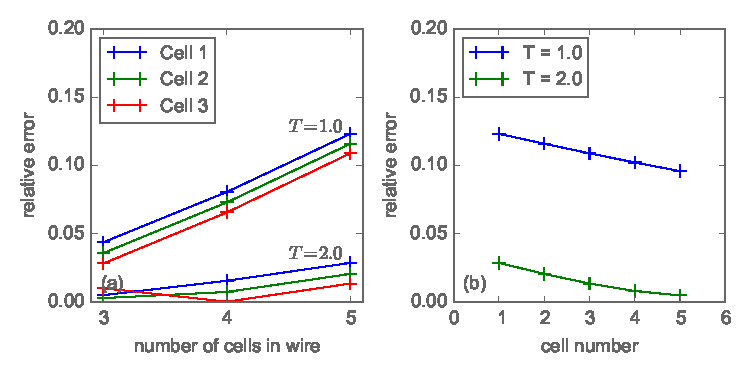
\includegraphics{ising_approximation3}
  \caption
  [The Ising approximation for three- to five-cell wires]
  {
  (a) The Ising model's relative error of the cell polarization for three-cell
  to five-cell charge-neutral wires at two different temperatures. The longer
  the wire the larger becomes the error. The error is no longer well controlled.
  (b) The Ising model's relative error for each cell's polarization in a
  five-cell charge-neutral wire. For the chosen parameters the error decreases
  along the wire. At least for the output polarization, the effect of a growing
  error with increasing wire length is therefore compensated.
  }
  \label{fig:ising_approximation3}
  % parameters: V1 = 100, boa = 3, P_D = 0.1, q = 0.5; 5 cells
\end{figure}
%

In this chapter we introduced and established three approximations for QCA
systems: the fixed charge, the bond, and the Ising model. We usually use the
fixed charge model as the starting point, without further explicit verification.
In principle, whether the fixed charge approximation holds for a chosen set of
parameters, has to be checked for each potential QCA implementation on a case by
case basis. If the fixed charge model is not applicable, then there is also
generally no hope of implementing QCA on the given experimental system. We
generally assume doubly occupied states to be sufficiently gapped out and put
$U$ at infinity. The bond approximation is then a very good description of QCA
systems at high temperatures. It starts breaking down when the temperature
becomes comparable to the singlet-triplet splitting, and therefore for small
$V_1$ and too large cell-cell distances. While it is conceptually deeply
rewarding to map QCA to an Ising system, we have seen the Ising approximation to
be difficult to handle for practical calculations. It is only valid in a
relatively small parameter window, at least for moderate system parameters, and
great care has to be taken with its application. Generally speaking, both the
bond and the Ising approximation become exact in the same limits---large $V_1/t$
and small (but not too small) cell-cell distances. Not coincidentally, those are
the limits where the QCA approach works best, as we will find out in the next
chapter. Both approximations are useless for low-temperature calculations and
for ground state properties we thus have to rely on the fixed charge model,
which, however, only allows system sizes of up to three cells. We will use the
bond model for most of our QCA characterization work at finite temperature. With
system sizes of up to six cells it already allows for some interesting insights.
The Ising model is problematic and we will employ it sparingly and only to look
at larger structures such as gates.
% TODO: mention again that Ising is the same as the two-state-approximation used
% in the literature (?)

% TODO: I should maybe work out in more detail how bond and Ising are different
% --- i.e. why is Ising problematic, but not the bond approximation? Both are
% valid in some parameter window, and the size of that window in only relative
% to the other parameters. Maybe it would be sufficient to be less dramatic
% about the Ising model. Of course, my discussion here is already coloured,
% because I already know where, for which parameters QCA will work and where it
% won't.
%
% TODO: I could also argue that the Ising approximation is a more complex
% approximation (i.e. an effective model) and therefore more tricky / involved
% than the bond approximation.
%
% TODO: Include partition function argument / explanation somewhere?
% TODO: good argument why there are two degenerate ground states for the bond
% model? (triplet, symmetry argument?)
% TODO: Is there a better explanation why bond chooses triplet and Ising singlet
% states?
% TODO: mention two sets of conditions (energy gap and temperature related) for
% Ising model?
% TODO: maybe explain somewhere: Ising weirdness is not a shortcoming of our
% derivation, but a consequence of pressing QCA in a two-state basis
